\chapter{Introduction}
\label{cha:introduction}

This chapter introduces the concepts of allostery in proteins, the protein structural ensemble, normal mode analysis, structural prediction of allostery, protein kinases and cyclin-dependent kinase 2 (CDK2).
Some of this introduction has been written as a review (cite).


\section{Normal mode analysis}




\section{Protein kinases}

Protein kinases regulate almost all aspects of cellular physiology, from proliferation and generation of biomass to gene expression and protein production \cite{Manning2002}.
In addition to medical benefits, regulation of kinase activity in mammalian cells is important in industrial production of biomolecules of high value, for example to prevent apoptosis and maximise yield.
In order to modulate kinase activity we need to develop specific regulators of protein kinase function, a process that is complicated by the conserved catalytic architecture of the huge range of protein kinases found in nature \cite{Muller2015}.
One way to achieve kinase regulation with enhanced selectivity is through isolation of allosteric regulators, as their target sites are likely to be less structurally conserved across the protein kinase family.

A few notable examples have highlighted this potential \cite{Gavrin2013}.
Serine/threonine-protein kinase Chk1 has been the target of high-throughput screening efforts \cite{Converso2009}, leading to the discovery of an inhibitor that binds 13 \AA\ from the active site.
This inhibitor binds largely to the protein surface, with part sliding into a narrow hydrophobic cleft, indicating that unexpected sites on proteins may reveal allosteric properties.
Despite locating the allosteric binding site, the mechanism for inhibition is not currently known \cite{Vanderpool2009}.
Study of the tyrosine-protein kinase Abl1 has revealed an inhibitor that binds far from the ATP binding site \cite{Zhang2010, Yang2011}.
Binding of the modulator leads to changes in structural dynamics at the ATP binding site, preventing the binding of ATP and leading to inhibition.
Other targets for which allosteric modulators have been discovered include the MAP kinases \cite{Comess2011} and CDK2 \cite{Betzi2011}.
Modulators such as these that bind protein kinases at sites removed from the ATP-binding site are known as type IV inhibitors.
The binding sites of the above type IV inhibitors, along with others, are shown on the conserved protein kinase structure in Figure~\ref{fig:kinase_mods}.
Type I inhibitors are directly-competitive with ATP as they target the active conformation.
Type II inhibitors bind to the DFG-out conformation and occupy the ATP-binding site and the surrounding hydrophobic region.
Type III inhibitors bind the hydrophobic cleft adjacent to the ATP-binding site but do not bind the ATP-binding site itself.
A novel class of inhibitors, the type V bisubstrate and bivalent inhibitors, has emerged recently \cite{Lamba2012}.
For example, a bivalent inhibitor was designed for a tyrosine kinase that binds to the ATP-binding site and to the regulatory domain SH3 simultaneously via a linker \cite{Hill2009}.
Such binding is able to have both high selectivity and high affinity.
The recent discovery of such sites and the conserved architecture of the eukaryotic protein kinases suggest there are many allosteric sites, particularly for type IV and type V inhibitors, yet to be discovered.

Numerous examples of allosteric kinases are listed in the AlloSteric Database (ASD) \cite{Shen2016}, a resource set up in 2011 that now contains over 1,400 allosteric proteins and over 70,000 allosteric modulators.
The allosteric proteins in the ASD are those that have experimental evidence for allostery.
The increasing number of entries in this database shows that a large number of proteins have allosteric character, and implies that many proteins have allosteric character yet to be discovered.


\begin{figure}
\centering

\includegraphics[width=\textwidth]{images/kinase_mods}

\caption{Binding sites of known type IV allosteric inhibitors are shown in purple on the cAMP-dependent protein kinase (PKA) structure (PDB ID 1ATP).
The ATP binding site is shown in yellow.
Figure reproduced from Lamba and Ghosh (2012) \cite{Lamba2012}.}

\label{fig:kinase_mods}
\end{figure}


\section{Cyclin-dependent kinase 2}

CDK2 is a protein kinase essential for the G1/S phase transition in the cell cycle \cite{Peyressatre2015}.
It associates with, and is regulated by, cyclins.
It has been a major target of drug discovery efforts due to its essential role.
